We evaluate the proposed methods by comparing them against naive baselines in terms of computational cost and scalability. 
Experiments were conducted on two real Bayesian networks, \cancerNetwork{} and \childNetwork{}, obtained from the \texttt{bnlearn} repository. Both were used as data distributions and as causal DAGs. The \childNetwork{} network was modified into a polytree by removing edges that introduce cycles in the underlying undirected graph.
Datasets were generated by sampling from these networks, and decision trees were trained accordingly. For ASV computation, the prediction variable was removed from the network to avoid trivial inference. To analyze the performance of the algorithms that compute the equivalence classes of topological sorts we also created artificial networks shaped as (1) Balanced binary trees, (2) Naive-bayes distributions, and (3) Trees composed by merging directed paths on their root (what we call \texttt{multiplePaths}).\footnote{All experiments were run on an Intel i5-7500 CPU @ 3.40GHz with 16 GB of RAM, using Ubuntu 22.04 and Python 3.12. The main libraries used were \texttt{pgmpy}, \texttt{sklearn}, \texttt{networkx}, and \texttt{shap}.}

\vspace{-3mm}

\paragraph{Equivalence Classes vs. Topological Orders} We compare the naive ASV computation based on iteratingg all topological orders with our approach based on equivalence classes. The key quantities are the sizes of $\topo(G)$ and $\Lambda^x_{G}$, as well as the cost of constructing each set.

\begin{figure}[ht]
	\centering
	\begin{subfigure}[b]{0.49\linewidth}
		\centering
		
\includegraphics[width=\linewidth]{img/equivalentClassesVsToposorts.png}
		\caption{Number of equivalence classes vs. topological orders.}
		\label{fig:equivalenceClassesVsToposortsNumberPlot}
	\end{subfigure}
	\hfill
	\begin{subfigure}[b]{0.49\linewidth}
		\centering
		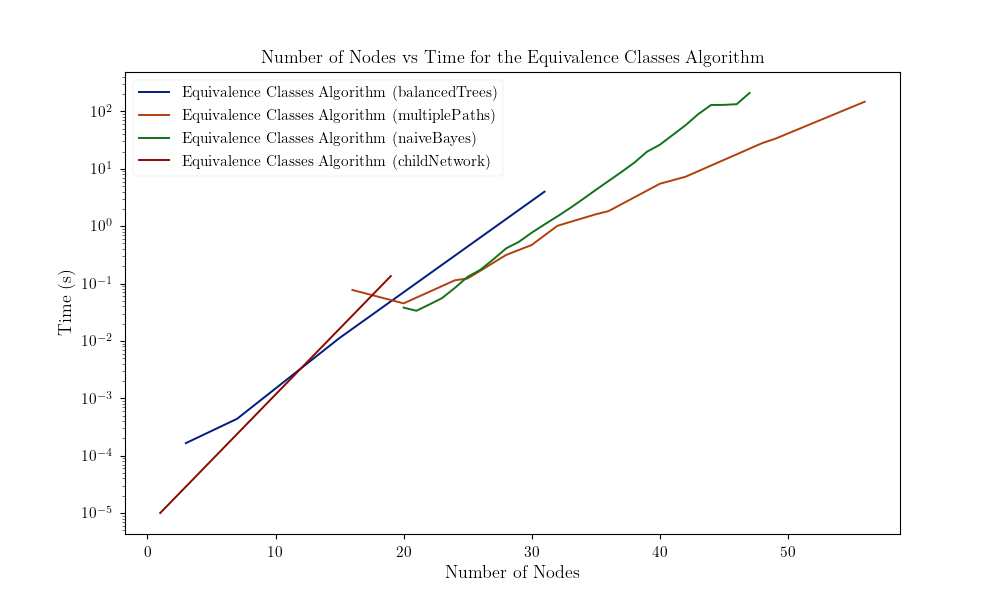
\includegraphics[width=\linewidth]{img/equivalentClasses_timevsNodes.png}
		\caption{Runtime for computing equivalence classes.}
		\label{fig:equivalenceClassesTimePlot}
	\end{subfigure}
	\label{fig:eq_vs_topo_combined}
\end{figure}

Figure~\ref{fig:equivalenceClassesVsToposortsNumberPlot} shows that the number of equivalence classes grows significantly slower than the number of topological orders. For instance, in \childNetwork{}, the graph has $7.41\times10^{11}$ topological orders but only around $2003$ equivalence classes on average\footnote{We mean the average value of $|\Lambda^x_G|$ over the set of features.}. Similar gaps are observed in balanced trees, where the difference can reach several orders of magnitude.
At the same time, the cost of computing equivalence classes remains moderate for graphs of practical size, typically under a few seconds. For example, in \childNetwork{}, all equivalence classes are computed in less than one second.
This reduction directly decreases the number of evaluations of the characteristic function, making the equivalence class approach substantially more efficient.

\vspace{-3mm}

\paragraph{Performance of Equivalence Class Algorithms} We now analyze the cost of computing equivalence classes.
As shown in Figure~\ref{fig:equivalenceClassesTimePlot}, the computation remains efficient for moderate graph sizes, typically under a few seconds. However, as graph size increases, the runtime grows alongside the number of equivalence classes.
We can see in Figure~\ref{fig:timeVsEquivClasses} that the runtime is strongly correlated with the number of equivalence classes. This is useful not only for explaining the observed growth, but also from a practical point of view. Since we also have a procedure to count the number of equivalence classes beforehand, we can use it as a rough predictor of the computational cost of the exact algorithm before actually running it.

\begin{figure}[ht]
	\centering
	
	\begin{subfigure}[t]{0.48\linewidth}
		\vspace{0pt}
		\centering
		
\includegraphics[width=\linewidth]{img/equivalentClassesVsAllToposorts_time.png}
		\caption{Runtime comparison between computing equivalence classes and enumerating all topological orders.\footnotemark}
		\label{fig:equivalenceClassesVsToposortsTimePlot}
	\end{subfigure}
	\hfill
	\begin{subfigure}[t]{0.48\linewidth}
		\vspace{0pt}
		\centering
		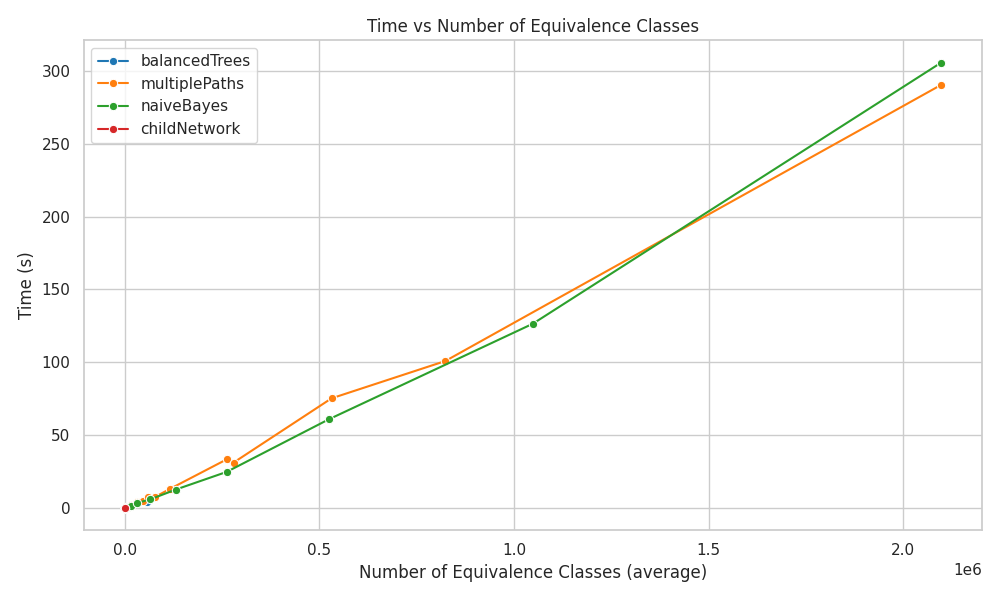
\includegraphics[width=\linewidth]{img/time_vs_equiv_classes.png}
		\caption{Runtime as a function of the number of equivalence classes.}
		\label{fig:timeVsEquivClasses}
	\end{subfigure}
	\label{fig:runtime_experiments}
\end{figure}
\footnotetext{To estimate runtime, we measured the time required to generate the first 1000 topological orders and extrapolated using the total number of orders in each graph, since full execution was not computationally feasible.}

Figure~\ref{fig:equivalenceClassesVsToposortsTimePlot} highlights the main advantage of our approach. While enumerating all topological orders quickly becomes infeasible (e.g., requiring days for large graphs), computing equivalence classes remains tractable.

\vspace{-3mm}

\paragraph{Sampling-Based Approximation of Topological Orders} We now evaluate the sampling-based approach.

\begin{figure}[H]
	\centering
	
	\begin{subfigure}[t]{0.32\linewidth}
		\vspace{0pt}
		\centering
		\small
		\setlength{\tabcolsep}{4pt}
		\renewcommand{\arraystretch}{1.1}
		\begin{tabular}{|r|r|}
			\hline
			\textbf{\# Samples} & \textbf{Time (s)}\\
			\hline
			100   & 0.9270 \\
			1000  & 1.1170 \\
			10000 & 4.7170 \\
			20000 & 7.7170 \\
			30000 & 10.8387 \\
			\hline
		\end{tabular}
		\caption{Sampling times for topological orders in \childNetwork{} using our developed algorithm.}
		\label{fig:samplingTimesTopoSorts}
	\end{subfigure}
	\hfill
	\begin{subfigure}[t]{0.64\linewidth}
		\vspace{0pt}
		\centering
		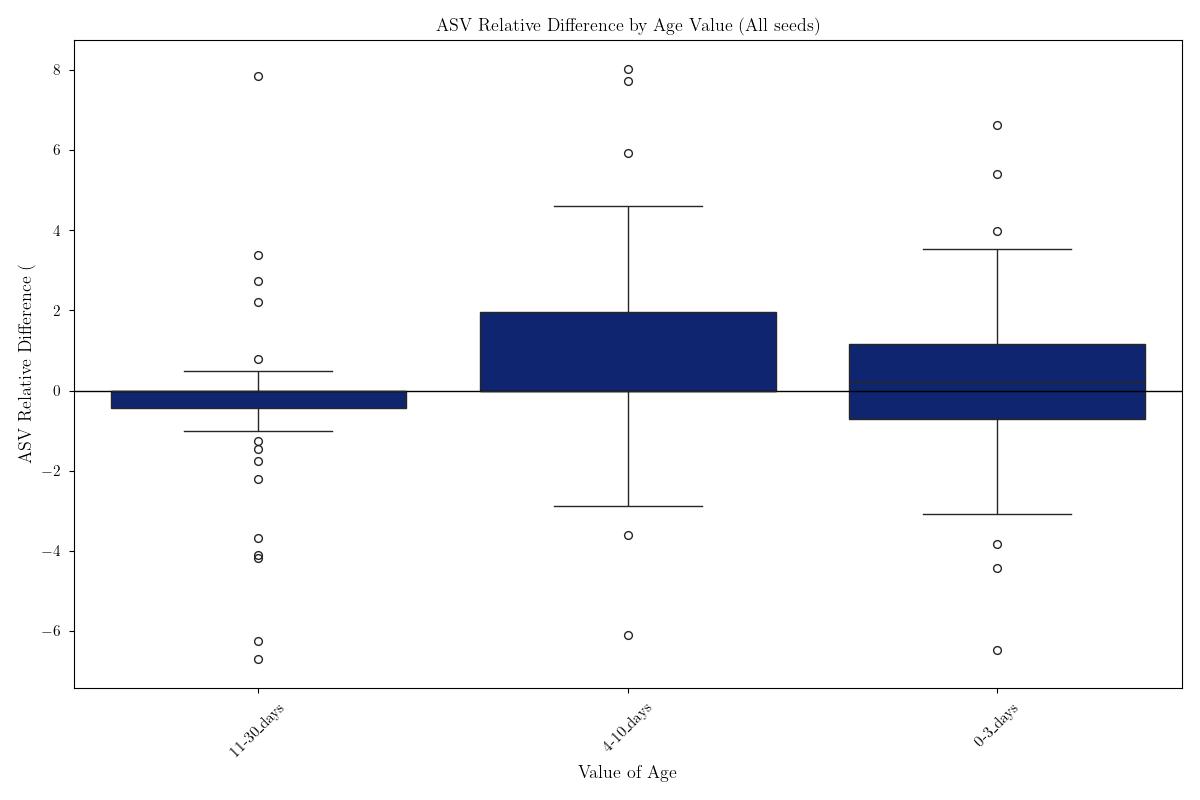
\includegraphics[width=0.80\linewidth]{img/ChildAllSeedsASVBoxplot.png}
		\caption{Relative error between approximate and exact ASV values in \childNetwork{}.}
		\label{fig:boxplotASVApproximateDifferences}
	\end{subfigure}
	\label{fig:sampling_results_combined}
\end{figure}

Table~\ref{fig:samplingTimesTopoSorts} shows that when using our algorithm the sampling remains efficient even for large numbers of samples. Moreover, the runtime is not linear in the number of samples, as multiple candidates are generated simultaneously during recursive calls due to our efficient implementation.
We conclude that in the bounded-degree setting (observe that in all the examples considered here most nodes have small degree) our algorithm is more efficient than the alternative options such as \cite{HUBER2006420}. Nevertheless, we recall that their algorithm is more general, as it applies beyond polytrees and runs in polynomial time.

Finally, we evaluate the approximation error of ASV using sampled orders. Figure~\ref{fig:boxplotASVApproximateDifferences} shows that using 1000 samples yields an average relative error of around $8\%$. Larger ASV values exhibit smaller relative error, while larger deviations correspond to very small true values.
These results indicate that sampling provides a practical trade-off between accuracy and computational cost.

\vspace{-3mm}

\paragraph{Remarks on Mean Prediction Computation} In our experiments, the cost of evaluating the characteristic function is not the dominant factor. This happens because for decision trees under Bayesian Network distributions with a polytree structure mean prediction can be computed exactly in an efficient way. In general models this might not be the case, but nonetheless due to Proposition~\ref{prop:sampling_to_compute_ASV} if sampling is used instead of exact computation the overall error of the approximation should not be extremely bad.